\documentclass[12pt]{article}

% feina a fer per al curs 2010-2011
% 1) l'exercici proposat de maximitzar una funció de dues variables és difícil i cal treballar-lo. Mirar bé el mètode d'steepest descent i el de Newton Raphson (els dos proposats a l'exercici). Mirar també d'entendre correctament el mètode d'optimitzar la funció de Davidson. Mirar una bona explicació a http://linneus20.ethz.ch:8080/1_5_3.html#SECTION00253100000000000000 Fer un dibuis que mostri el concepte de "constant norm", entès com un radi determinat al voltant d'x, un radi donat per l'stepsize. És prou entendor així
\usepackage{framed}
\usepackage{url}
\usepackage{ifthen}
\usepackage{longtable}
\usepackage{fancyvrb}
\usepackage[catalan]{babel}
\usepackage{cancel}
\usepackage{enumitem}
\usepackage[thinc]{esdiff}

%\usepackage[utf8]{inputenc}
\usepackage[catalan]{babel}
\usepackage{lmodern}
\usepackage{diagbox}
\usepackage{amsmath,amsthm,amsfonts,amssymb,amscd}
%\newcommand*\diff{\mathop{}\!\mathrm{d}}
%\newcommand*\Diff[1]{\mathop{}\!\mathrm{d^#1}}
\usepackage[]{systeme}
\usepackage[arrowdel]{physics}
\usepackage{multirow,booktabs}
\usepackage[dvipsnames,table]{xcolor}
%\usepackage{fullpage}
\usepackage{lastpage}
\usepackage{graphicx}
\graphicspath{{../figures/}}

\usepackage{enumitem}
\usepackage{fancyhdr}
\setlength{\headheight}{14pt}
\usepackage{mathrsfs}
\usepackage{wrapfig}
\usepackage{setspace}
\usepackage{calc}
\usepackage{multicol}
\usepackage{textcomp}
\usepackage{gensymb}
\usepackage{listings}
\usepackage{siunitx}

\usepackage{cancel}
%\usepackage[retainorgcmds]{IEEEtrantools}
\usepackage[margin=3cm]{geometry}
\usepackage{amsmath}
\newlength{\tabcont}
\setlength{\parindent}{0.0in}
\setlength{\parskip}{0.05in}
\usepackage{empheq}
\usepackage{framed}
\usepackage{mdframed}

\usepackage[most]{tcolorbox}
% \usepackage{chemfig,chemmacros,chemnum}
% \usepackage{chemformula}

%\usepackage{unicode-math}

\usepackage{tcolorbox}
\usepackage{url}
  \let\oldurl\url
\usepackage{hyperref}
  \let\linkurl\url
  \let\url\oldurl

% \usepackage[
% backend=biber,
% citestyle=numeric-comp
% ]{biblatex}
% \addbibresource{/Users/556079/Documents/teaching.bib}


%\chemsetup[chemformula]{format=\sffamily}
%\renewcommand*\printatom[1]{\ensuremath{\mathsf{#1}}}
%\setatomsep{2em}
%\setdoublesep{.6ex}
%\setbondstyle{semithick}
%\colorlet{shadecolor}{orange!15}
% \parindent 0in
% \parskip 12pt
% \geometry{margin=1in, headsep=0.25in}
% \theoremstyle{definition}
% \newtheorem{defn}{Definition}
% \newtheorem{reg}{Rule}
% \newtheorem{exer}{Exercise}
% \newtheorem{note}{Note}
%\RequirePackage{mathrsfs}
%\RequirePackage[psamsfonts]{amsfonts} %for Y&Y BSR AMS fonts
\RequirePackage{amsmath,amsfonts,amsthm,amssymb}
\RequirePackage{setspace}
\RequirePackage{fancyhdr}
\RequirePackage{lastpage}
\RequirePackage{extramarks}
\RequirePackage{chngpage}
\RequirePackage{soul}


\usepackage{graphicx}
\usepackage{multicol}
\usepackage{hyperref}
\usepackage{makecell}
\usepackage{fancybox}

%\RequirePackage[dvipsnames]{xcolor}
%\RequirePackage{graphicx,float,wrapfig}
\RequirePackage{pgf,tikz}
\usepackage{pgfplots}
%\usetikzlibrary{arrows,automata}
%\RequirePackage{pstricks}
%\RequirePackage[text]{amsthm}
%\RequirePackage{array}
%\RequirePackage{amscd}
%\RequirePackage{array}\RequirePackage{dcolumn}
%\putfig{3.5truein}{PSfig1.3}{Peter's winnings in 40 plays of heads or tails.}{fig 1.3}

% \newcommand*{\DIRFig}{../../../../talks/figures}
% \newcommand{\barefig}[2]{\makebox{\includegraphics*[width=#2] {\DIRFig/#1}}}
% \newcommand{\putfig}[4]
% {\begin{figure}
% \centerline{\barefig{#2}{#1}}
% \caption{#3}
% \label{#4}
% \end{figure}}

\newcommand{\dif}{\, \mathop{}\!\mathrm{d}}
\newcommand{\dx}{\, dx}
\newcommand{\dy}{\, dy}
\newcommand{\dt}{\, dt}
\newcommand{\dth}{\, d\theta}
\newcommand{\dr}{\, dr}
\newcommand{\du}{\, du}
\newcommand\uvec[1]{\textbf{#1}}
\newcommand{\iu}{\hat{\uvec{i}}}
\newcommand{\ju}{\hat{\uvec{j}}}
\newcommand{\ku}{\hat{\uvec{k}}}

% \newcommand{\emx}[1]{{\em{#1}\/}}
% \newcommand{\abin}{{\it ab initio}}
% \newcommand{\bs}{\boldsymbol}
% \newcommand{\citenum}{\cite}
% \newcommand{\dGo}{\ensuremath{\Delta G_0}}
% \newcommand{\dG}[2]{\ensuremath{\Delta G_{\rm #1}^{\rm #2}}}
% \newcommand{\dX}[3]{\ensuremath{\Delta #1_{\rm #2}^{\rm #3}}}
% \newcommand{\ddgo}[1]{\ensuremath{\Delta \Delta G_{\rm solv}^{\rm #1}}}
% \newcommand{\ddgstarcat}{\ensuremath{\Delta \Delta g^{\ddagger}_{\rm cat}}}
% \newcommand{\ddgstar}{\ensuremath{\Delta \dgstar}}
% \newcommand{\ddgt}[2]{\ensuremath{\Delta \Delta G_{\rm solv}^{\rm #1, \rm #2}}}
% \newcommand{\ddsstarprime}{\ensuremath{(\Delta \dsstar)'}}
% \newcommand{\deltaepsel}{\ensuremath{\Delta \varepsilon_{\rm el}}}
% \newcommand{\deltaeps}{\ensuremath{\Delta \varepsilon}}
% \newcommand{\dgab}[2]{\ensuremath{\Delta g_{\rm #1}^{\rm #2}}}
% \newcommand{\dga}[1]{\ensuremath{\Delta g_{\rm #1}}}
% \newcommand{\dgb}[1]{\ensuremath{\Delta g^{\rm #1}}}
% \newcommand{\dgcage}{\ensuremath{\Delta g_{\rm cage}}}
% \newcommand{\dgcat}{\ensuremath{\Delta g_{\rm cat}}}
% \newcommand{\dgsoltsatsa}{\ensuremath{\dgsol (\rm TSA)_{\rm TSA}}}
% \newcommand{\dgsoltstsa}{\ensuremath{\dgsol (\rm TS)_{\rm TSA}}}
% \newcommand{\dgsoltsts}{\ensuremath{\dgsol (\rm TS)_{\rm TS}}}
% \newcommand{\dgsol}{\ensuremath{\Delta G_{\rm sol}}}
% \newcommand{\dgstarcage}{\ensuremath{\dgstar_{\rm cage}}}
% \newcommand{\dgstarcat}{\ensuremath{\dgstar_{\rm cat}}}
% \newcommand{\dgstarw}{\ensuremath{\dgstar_{\rm w}}}
% \newcommand{\dgstar}{\ensuremath{\Delta g^{\ddagger}}}
% \newcommand{\dgw}{\ensuremath{\Delta g_{\rm w}}}
% \newcommand{\dg}[2]{\ensuremath{\Delta g_{\rm #1}^{\rm #2}}}
% \newcommand{\dino}{\texttt{DINO}}
% \newcommand{\dsstarcageprime}{\ensuremath{(\dsstarcage)'}}
% \newcommand{\dsstarcage}{\ensuremath{\dsstar_{\rm cage}}}
% \newcommand{\dsstarcatprime}{\ensuremath{(\dsstarcat)'}}
% \newcommand{\dsstarcat}{\ensuremath{\dsstar_{\rm cat}}}
% \newcommand{\dsstarwprime}{\ensuremath{(\dsstarw)'}}
% \newcommand{\dsstarw}{\ensuremath{\dsstar_{\rm w}}}
% \newcommand{\dsstar}{\ensuremath{\Delta S^{\ddagger}}}
% \newcommand{\eg}{{\it e.g.}}
% \newcommand{\etal}{{\it et al.}}
% \newcommand{\gamess}{\texttt{GAMESS}}
% \newcommand{\gauss}{\texttt{GAUSSIAN} 98}
% \newcommand{\golpe}{\texttt{GOLPE}}
% \newcommand{\grid}{\texttt{GRID}}
% \newcommand{\ie}{{\it i.e.}}
% \newcommand{\ith}{{\it i}$^{\rm th}$\ }
% \newcommand{\kbt}{\ensuremath{k_{\rm B} T}}
% \newcommand{\kb}{\ensuremath{k_{\rm B}}}
% \newcommand{\kcage}{\ensuremath{k_{\rm cage}}}
% \newcommand{\kcatkm}{\ensuremath{k_{\rm cat}/K_{\rm M}}}
% \newcommand{\kcat}{\ensuremath{k_{\rm cat}}}
% \newcommand{\km}{kcal mol$^-1$}
% \newcommand{\knon}{\ensuremath{k_{\rm non}}}
% \newcommand{\kw}{\ensuremath{k_{\rm w}}}
% \newcommand{\mepsim}{\texttt{MEPSIM}}
% \newcommand{\mgp}[1]{\marginpar{\scriptsize{#1}}}
% \newcommand{\mipsim}{\texttt{MIPSIM}}
% \newcommand{\mola}{\texttt{MOLARIS}}
% \newcommand{\msms}{\texttt{MSMS}}
% \newcommand{\pdras}{p21$^{\rm ras}$}
\newcommand{\rgran}{\ensuremath{\mathbb{R}}}
\newcommand{\rx}[2]{\ensuremath{#1_{\rm #2}}}
\newcommand{\vs}{{\it vs.}}
\newcommand{\z}[1]{\ensuremath{\mathbf{#1}}}
\newcommand{\composed}[2]{#1\mathbin\circ #2}
\newcommand{\wrt}[1]{{\mbox{\scriptsize w.r.t. \( #1 \)} }}
\newcommand{\polyspace}{\mathcal{P}}
\newcommand{\matspace}{\mathcal{M}}
%\newcommand{\C}{\mathbb{C}}
\newcommand{\N}{\mathbb{N}}
\newcommand{\Q}{\mathbb{Q}}
\newcommand{\Z}{\mathbb{Z}}
\renewcommand{\Re}{\mathbb{R}}
\newcommand{\rtres}{\ensuremath{\Re^3}}
\newcommand{\union}{\cup}
\newcommand{\dotprod}{\cdot}
\newcommand*\pkg[1]{\textsf{#1}}

%\def\checkmark{\tikz\fill[scale=0.4](0,.35) -- (.25,0) -- (1,.7) -- (.25,.15) -- cycle;}


\newcommand{\trans}[1]{{#1}^{\ensuremath{\mathsf{T}}}} % transpose
\newcommand{\nbyn}[1]{\ensuremath{#1 \! \times \! #1 }}
\newcommand{\nbym}[2]{#1 \! \times \! #2 }       % Use in math mode.
\newcommand{\cat}[2]{#1\!\mathbin{\raise.6ex\hbox{\( {}^\frown \)}}\!#2}
\newcommand{\generalmatrix}[3]{ %arg1: low-case letter, arg2: rows, arg3: cols
               \left(
                  \begin{array}{cccc}
                    #1_{1,1}  &#1_{1,2}  &\ldots  &#1_{1,#2}  \\
                    #1_{2,1}  &#1_{2,2}  &\ldots  &#1_{2,#2}  \\
                              &\vdots                         \\
                    #1_{#3,1} &#1_{#3,2} &\ldots  &#1_{#3,#2}
                  \end{array}
               \right)  }
\newcommand{\colvec}[1]{\begin{pmatrix} #1 \end{pmatrix}}
\newcommand{\pr}[1]{\ensuremath{\mathrm{Pr}(#1)}}
\newcommand{\rep}[2]{ {\rm Rep}_{#2}(#1) }
\newcommand{\mapsunder}[1]{\stackrel{#1}{\longmapsto}}
\newcommand{\map}[3]{\mbox{$#1\colon #2\to #3$}}
\newcommand{\identity}{\mbox{id}}
\newcommand{\stdbasis}{{\cal E}}
\newcommand{\sequence}[1]{ \langle#1\rangle }
\newcommand{\spacer}{\rule[-3mm]{0mm}{8mm}}
\newcommand{\email}[1]{\url{#1}}
\newcommand{\zero}{\vec{0}}
\newcommand{\proj}[2]{\mbox{proj}_{#2}({#1}) }
%\AtBeginDocument{\newlength{\heightofcdot}
%\newlength{\widthofcdot}
%\settoheight{\heightofcdot}{$\cdot$}
%\settowidth{\widthofcdot}{$\cdot$}
%\newsavebox{\dotprodcircle}
%\savebox{\dotprodcircle}{\includegraphics{dotprod.1}}
%\newcommand{\dotprod}{\mathbin{\raisebox{.5\heightofcdot}{%
%          \makebox[\widthofcdot]{$\smash{\usebox{\dotprodcircle}}$}}}}}
\newcommand{\spanof}[1]{\relax [#1\relax ]} % no optional argument!
\newcommand{\set}[1]{\mbox{$\{#1\}$}} \newcommand{\suchthat}{\bigm|}
\newcommand{\deter}[1]{ \mathchoice{\left|#1\right|}{|#1|}{|#1|}{|#1|} }
\newcommand{\secuence}[1]{ \langle#1\rangle }
\newcommand{\basis}[2]{\secuence{\vec{#1}_1,\ldots,\vec{#1}_{#2}}}



%--------linsys
%  Use as \begin{linsys}{3}
%           x &+ &3y &+ &a &= &7 \\
%           x &- &3y &+ &a &= &7
%         \end{linsys}
% Remark: TeXbook pp. 167-170 says to put a medmuskip around a +; and that's
% 4/18-ths of an em.  Why does 2/18-ths of an em work?  I don't know, but
% comparing to a regular displayed equation suggests it is right.
% (darseneau says LaTeX puts in half an \arraycolsep.)
\newenvironment{linsys}[2][m]{%
\setlength{\arraycolsep}{.1111em} % p. 170 TeXbook; a medmuskip
\begin{array}[#1]{@{}*{#2}{rc}r@{}}
}{%
\end{array}}


%\newtheorem{teorema}{Teorema}
%\newtheorem{exercici}{Exercici}
%\newtheorem{definicio}{Definici\'o}
%\newtheorem{theorem}{Theorem}
\newtheorem{exercise}{Exercise}
%\newtheorem{definition}{Definition}

\newcounter{EXMP}
\newenvironment{EXMP}[1][]{\definecolor{shadecolor}{rgb}{0.6,0.6,0.6}
							\begin{shaded}\refstepcounter{EXMP}\par\medskip\noindent%
   							\textbf{EXAMPLE~\theEXMP. #1} \rmfamily}
   							{\end{shaded}\medskip}

\newcounter{BOXT}
\newenvironment{BOXT}[1][]{\definecolor{shadecolor}{rgb}{0.8,0.8,0.8}
							\begin{shaded}\refstepcounter{BOXT}\par\medskip\noindent%
   							\textbf{BOX~\theBOXT. #1} \rmfamily}
   							{\end{shaded}\medskip}

\parskip 4mm


\usepackage{makeidx}
\makeindex


% margins
\topmargin=-0.45in      %
\evensidemargin=0in     %
\oddsidemargin=0in      %
\textwidth=6in        %
\textheight=8.5in       %
\headsep=0.25in         %

% header and footer
\pagestyle{fancy}       %                %
\cfoot{
\includegraphics[width=4.8cm]{FCTE}}                %
\rfoot{\thepage}        %
\renewcommand\headrulewidth{0.4pt}   %
\renewcommand\footrulewidth{0.4pt}   %

%\setcounter{section}{-1}

\theoremstyle{definition}
\newtheorem{thm}{Theorem}
\newtheorem{dfn}{Definition}
\newtheorem{lem}{Lemma}
\newtheorem{prp}{Proposition}



%%%%%%%%%%%%%%%%%%%%%%%%%%%%%%%%%%%%%%%%%
%%%%%%%%%%%%%%%%%%%%%%%%%%%%%%%%%%%%%%%%%
% lecturer or student text
% in principle the lecturer text includes some examples to be done in the c lass
\newboolean{LECT}
\setboolean{LECT}{false}
\setboolean{LECT}{true}
%%%%%%%%%%%%%%%%%%%%%%%%%%%%%%%%%%%%%%%%%
%%%%%%%%%%%%%%%%%%%%%%%%%%%%%%%%%%%%%%%%%

\newenvironment{lect}{ %
	\definecolor{shadecolor}{rgb}{1.0,0.8,0.8} %
	\begin{shaded} %
	\textcolor{BrickRed}{\bf Resultat\\}%

} %
{ %
	\end{shaded}
} %

\newcommand{\lct}[1]{\ifthenelse{\boolean{LECT}}{\begin{lect} #1 \end{lect}}{}}



%%%%%%%%%%%%%%%%%%%
% ANGLÈS
%%%%%%%%%%%%%%%%%%%

%\newcommand{\problemName}{}%
%\newcounter{problemCounter}%
%\newenvironment{problem}[1][Problem \arabic{problemCounter}]%
%	{\stepcounter{problemCounter}%
%		\renewcommand{\problemName}{#1}%
%		\section*{\problemName}%
%		\nobreak\extramarks{\problemName}{\problemName continued on next page\ldots}\nobreak%
%		\nobreak\extramarks{\problemName (continued)}{\problemName continued on next page\ldots}\nobreak}%
%	{\nobreak\extramarks{\problemName (continued)}{\problemName continued on next page\ldots}\nobreak%
%		\nobreak\extramarks{\problemName}{}\nobreak}%

\newenvironment{example}{ %merges with the question content
} %


\newenvironment{introduction}{ %
	\definecolor{shadecolor}{rgb}{1.0,1.0,0.8} %
	\begin{shaded} %
	% \textcolor{BrickRed}{\bf Introduction\\}%
} %
{ %
	\end{shaded}
} %


%%%%%%%%%%%%%%%%%%%
% CATALÀ
%%%%%%%%%%%%%%%%%%%
\newtheorem{teorema}{theorem}
\newenvironment{definicio}{ %
	\definecolor{shadecolor}{rgb}{0.9,1.0,0.8} %
	\begin{shaded} %
	\textcolor{OliveGreen}{\bf Definicio\\}%
} %
{ %
	\end{shaded}
} %

%veure http://en.wikibooks.org/wiki/LaTeX/Advanced_Topics
\newcounter{myc}
%environment for exercises in the class notes
\newenvironment{exr}{ %
    \addtocounter{myc}{1}
	\definecolor{shadecolor}{rgb}{0.9,1.0,0.8} %
	\begin{shaded} %
	\textcolor{OliveGreen}{\bf Exercici \arabic{myc}\\}%
} %
{ %
	\end{shaded}
} %
%environment for questions in exams
\newenvironment{qst}{ %
    \addtocounter{myc}{1}
	\definecolor{shadecolor}{rgb}{0.9,1.0,0.8} %
	\begin{shaded} %
	\textcolor{OliveGreen}{\bf Qüestió \arabic{myc}\\}%
} %
{ %
	\end{shaded}
} %


\usepackage[lastexercise]{exercise}
% \renewcommand{\listexercisename}{\'{I}ndex d'exercicis}
% \renewcommand{\ExerciseListName}{Ex.}  % titol a cada exercici
% \renewcommand{\AnswerListName}{Soluci\'{o}}
% \renewcommand{\AnswerName}{Soluci\'{o} de l'exercici}
% \renewcommand{\ExerciseName}{Exercici}  % títol que apareix al llistat d'exercicis
% \renewcommand{\ExerciseHeaderTitle}{\ExerciseTitle \quad---\quad \medskip}
% \renewcommand{\ExerciseListHeader}{
%         \shadowbox*{
%                 \ExerciseHeaderDifficulty%
%                 \textbf{\ExerciseListName\ \ExerciseHeaderNB%
%                 \ --- \ \ExerciseHeaderTitle}%
%                 \medskip\ExerciseHeaderOrigin%
%                 \ignorespaces
%         }
% }

\makeatletter
% remove the faulty \expandafter
\patchcmd{\@@@ExeEnv}
  {\theExercise\ \expandafter}
  {\theExercise\ }
  {}{}
\patchcmd{\@@@ExeCmd}
  {\theExercise\ \expandafter}
  {\theExercise\ }
  {}{}
% remove \itshape
\patchcmd{\@@@ExeEnv}
  {\itshape}
  {}
  {}{}
\patchcmd{\@@@ExeCmd}
  {\itshape}
  {}
  {}{}
\makeatother
\usepackage{amsmath, amssymb, amsthm}

\usepackage[catalan]{babel}
\usepackage{graphicx}
\graphicspath{{../figures/}}

\begin{document}

\lstset{language=Matlab,%
    basicstyle=\color{red},
    breaklines=true,%
    morekeywords={matlab2tikz},
    keywordstyle=\color{blue},%
    morekeywords=[2]{1}, keywordstyle=[2]{\color{black}},
    identifierstyle=\color{black},%
    stringstyle=\color{mylilas},
    commentstyle=\color{mygreen},%
    showstringspaces=false,%without this there will be a symbol in the places where there is a space
    numbers=left,%
    numberstyle={\tiny \color{black}},% size of the numbers
    numbersep=9pt, % this defines how far the numbers are from the text
    emph=[1]{for,end,break},emphstyle=[1]\color{red}, %some words to emphasise
    emph=[2]{word1,word2}, emphstyle=[2]{style},
}


\title{Exercicis Resolts \\ \large MATEMÀTIQUES I \\ Grau en Enginyeria Mecatrònica 
\author{Jordi Villà i Freixa}\thanks{Adreça electrònica: \texttt{jordi.villa@uvic.cat}}
\begin{center}
\includegraphics[width = 60mm]{FCTE}\end{center}}
\date{Darrera modificació: \today}
\maketitle

\tableofcontents
\newpage

Aquest és un llistat d'exercicis recollits de diverses fonts. Si hi detecteu algun error feu-me'l arribar i corregiré el document.
%
\begin{ExerciseList}
\section{Càlcul Integral}

\subsection{Integral indefinida}

%\begin{Exercise}[label=Ex1]
\Exercise[title=Substitució] $\int \frac{x}{\sqrt[5]{x^2+2}}dx$ (pista: usa la substició $t=x^2+2$)
%\end{Exercise}


\Answer
%  \begin{Answer}[ref=Ex1]

  Ens hem d'adonar que el numerador és proper a la derivada de l'argument de l'arrel del denominador. Això ens mostra que la funció primitiva tindrà l'aspecte d'una arrel, justament. Per mostrar-ho, la substitució a realitzar pot ser
  \[
    t=x^2+2 ; \; dt=2xdx; \; xdx=\frac{dt}{2}
  \]
  Quedant:
  \[
    \int \frac{x}{\sqrt[5]{x^2+2}}dx = \int \frac{1}{\sqrt[5]{t}}\frac{dt}{2} = \frac{1}{2} \int t^{-5} dt = \frac{1}{2} \frac{t^{-4}}{(-4)} = -\frac{1}{8t^4}
  \]

%\end{Answer}

%\begin{Exercise}[label=Ex2]
\Exercise[title=Substitució]
$\int \frac{1}{x^2 \sqrt{4-x^2}}dx$ (pista: usa dues substitucions consecutives)

%\end{Exercise}

%\begin{Answer}[ref=Ex2]
\Answer
Ens hem d'adonar que tenim una arrel de la forma $\sqrt{a^2-x^2}$. En aquests casos podem mirar de transformar l'arrel en quelcom del tipus $\sqrt{1-\sin^2{x}}$. Per tant, comencem plantejant el canvi
\[
  x=2\cos{t}; \; dx=-2\sin{t}dt
\]
I per tant:
\begin{eqnarray*}
  \int \frac{1}{x^2 \sqrt{4-x^2}}dx
  &=& \int \frac{-2\sin{t}}{4\cos^2{t}\sqrt{4-4\cos^2{t}}} dt = \int \frac{-2\sin{t}}{8\cos^2{t}\sqrt{1-\cos^2{t}}} dt\\
  &=& \int \frac{-2\sin{t}}{8\cos^2{t}\sqrt{\sin^2{t}}} dt = -\frac{1}{4} \int \frac{dt}{\cos^2{t}} dt=-\frac{1}{4} \tan{t}
\end{eqnarray*}

Ara podem desfer el canvi de variable fent $x=2\cos{t} \Rightarrow t=\arccos{\frac{x}{2}}$

\[
  \int \frac{1}{x^2 \sqrt{4-x^2}}dx=-\frac{1}{4} \tan{\arccos{\frac{x}{2}}}
\]

Ho podem deixar així o podem pensar en que si $\alpha=\arccos{\frac{x}{2}}$, segons el dibuix  $\tan{\arccos{\frac{x}{2}}}=\tan{\alpha}=\frac{\sqrt{1-\frac{x}{2}}}{\frac{x}{2}}$.

\begin{center}
  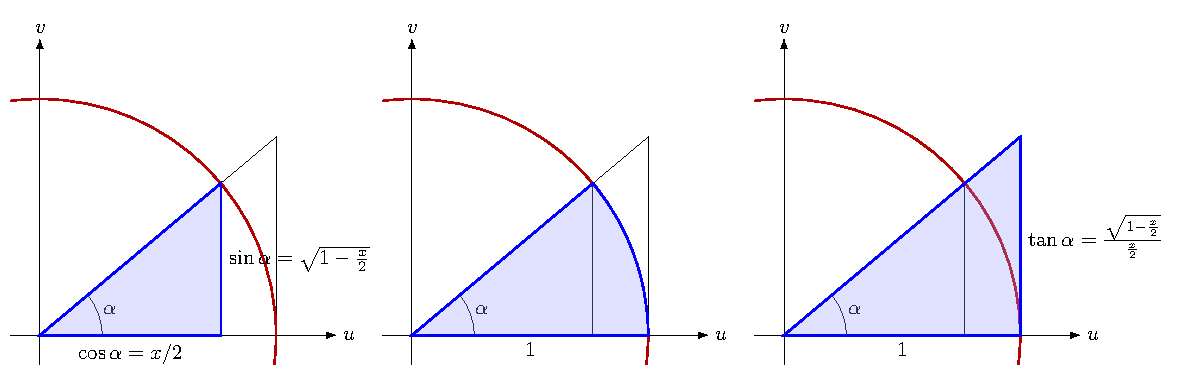
\includegraphics[width=0.8\textwidth]{Ex2unitcircle.pdf}
\end{center}

Per tant, per a $x=2\cos{t}$: 

\[
\int \frac{1}{x^2 \sqrt{4-x^2}}dx = -\frac{1}{4} \tan{t} = -\frac{1}{4}\frac{\sqrt{1-\frac{x}{2}}}{\frac{x}{2}}
\]

%\end{Answer}

\Exercise[title={$\int \frac{dx}{ax^2 + bx + c}$, amb denominador sense arrels reals (arctangent)}]
%\begin{Exercise}[label=Ex6]
  \vspace{5mm}
  $\int \frac{3}{x^2+2x+4} dx$
  

%\end{Exercise}

\Answer

%\begin{Answer}[ref=Ex6]

    En no haver zeros reals del polinoni del denominador ens cal usar l'estratègia de completar quadrats. Aquesta tècnica ens permet acostar l'expressió de la integral a la que tindria una primitiva arctangent.
    En general,
    \[
      ax^2+bx+c=a\left(x^2+\frac{b}{a}x+\frac{c}{a}\right)=a\left((x+r)^2+s^2\right)
    \]
    on es pot veure fàcilment que $r=\frac{b}{2a}$ i $s=\sqrt{\frac{c}{a}-\frac{b^2}{4a^2}}$.En aquest cas, $r=1$ i $s=\sqrt{3}$. Per tant:

    \[
      \int \frac{3}{x^2+2x+4} dx=3\int \frac{1}{(x+1)^2+(\sqrt{3})^2} dx\stackrel{(*)}{=} \frac{1}{\sqrt{3}}\arctan{\frac{x+1}{\sqrt{3}}}+C
    \]
    \begin{description}
      \item[$(*)$] Immediata, ja que $\int \frac{dx}{s^2+x^2}=\frac{1}{s}\arctan{\frac{x+r}{s}}+C$:
    \end{description}

\blacksquare



\Exercise[title={$\int \sin^m x \cos^n x dx$ amb \(m , n \in Z^+\) i $m$ o $n$ senar}]

%\begin{Exercise}[label=Ex3]

$\int \sin^5{x}dx$ 

%\end{Exercise}

\Answer
%  \begin{Answer}[ref=Ex3]

  Usarem que $\sin^2{x}+\cos^2{x}=1$ i l'expressió quedarà:

  \[
    I=\int \sin^5{x}dx = \int \left(1-\cos^2{x}\right)^2\sin{x}dx
  \]

  Veiem que, d'aquesta manera, ens queda una expressió que barreja sinus i cosinus, i sabem que un és la derivada de l'altre. Per tant, una bona substició és $t=\cos{x}; \; dt=-\sin{x}dx$
  \[
    I=\int \sin^5{x}dx = - \int \left(1-t^2\right)^2dt=-\frac{t^5}{5}+2 \frac{t^3}{3}-t+C= -\frac{\cos^5{x}}{5}+2 \frac{\cos^3{x}}{3}-\cos{x}+C
  \]


%\end{Answer}

\Exercise[title={$\int \sin^m x \cos^n x dx$ amb \(m , n \in Z^+\) i $m,n$ parells}]

%\begin{Exercise}[label=Ex4]

Avalúa la integral $\int{ \frac{1}{\sqrt{1-x^2}}dx}$

%\end{Exercise}

\Answer 
%\begin{Answer}[ref=Ex4]

    Considerem el canvi de variable
    \[x=\sin{u}; \; dx=\cos{u} du\].
    Per tant:
  \[
  I=\int \frac{1}{\sqrt{1-x^2}} dx = \int \frac{1}{\sqrt{1-\sin^2{u}}} \cos{u} du = \int \frac{1}{\sqrt{\cos^2{u}}} \cos{u}   du = \int du = u + C
  \]
  si desfem la substitució:
  \[
  I= \arcsin{x} + C
  \]

%\end{Answer}

\Exercise[title={Racional trigonomètrica $\int R(sin x, cos x) dx$}]

%\begin{Exercise}[label=Ex5]

Avalúa la integral $I = \int \frac{2}{1+3\cos{x}} dx$

(Pista: si $t = \tan{\theta/2}$, per raons trigonomètriques obtenim:

\begin{eqnarray*} \sin{\theta}&=&\frac{2t}{1+t^2}\\ \cos{\theta}&=&\frac{1-t^2}{1+t^2}\\ \tan{\theta}&=&\frac{2t}{1-t^2} \end{eqnarray*})





%\end{Exercise}

\Answer
%  \begin{Answer}[ref=Ex5]

    En els casos en que tenim \( I = \int \frac{1}{a+b\cos{x}} dx\) o bé \( I = \int \frac{1}{a+b\sin{x}} dx\) és pràctic usar la substitució \(t = \tan{x/2}\). Aleshores tenim:

    $$ dt=\frac{1}{2} \sec^2{\frac{x}{2}} dx = \frac{1}{2} \left( 1+\tan^2{\frac{x}{2}} \right) dx = \frac{1+t^2}{2} dx     $$

    i, per tant, \(dx=\frac{2}{1+t^2} dt\)

    \begin{eqnarray*}
    I &=& \int \frac{2}{1+3\cos{x}} dx = \int \frac{2}{(1+3\frac{1-t^2}{1+t^2})} \frac{2}{(1+t^2)} dt \\
    &=& 4 \int \frac{1}{1+t^2+3-3t^2}  dt =  4 \int \frac{1}{4-2t^2}  dt = \int \frac{1}{1-\left(\frac{t}{\sqrt{2}}\right)^2} dt
    \end{eqnarray*}

    i ara fem la substitució \(u=\frac{t}{\sqrt{2}}\) i \( du = \frac{dt}{\sqrt{2}}\)

    \begin{eqnarray*}
    I &=&  \int \frac{1}{1-\left(\frac{t}{\sqrt{2}}\right)^2} dt = \frac{1}{\sqrt{2}}  \int \frac{1}{1-u^2} du = \frac{1}{\sqrt{2}} \text{arctanh} \, {u} + C \\
    &=& \frac{1}{\sqrt{2}} \text{arctanh} {\frac{t}{\sqrt{2}}} + C =  \frac{1}{\sqrt{2}} \text{arctanh}  {\frac{\tan{x/2}}{\sqrt{2}}} + C
    \end{eqnarray*}

%\end{Answer}

\Exercise[title={$\int \sin^m x \cos^n x dx$ amb \(m , n \in Z^+\) i $m,n$ parells}]

%\begin{Exercise}[label=Ex6]

$\int \cos^4{x}dx$ (pista: per a funcions sinusoidals d'exponent parell, usa les expressions $\sin^2{x}=\frac{1}{2}(1-\cos{2x})$ o bé $\cos^2{x}=\frac{1}{2}(1+\cos{2x})$ per reduir l'exponent.)


%\end{Exercise}

\Answer

%\begin{Answer}[ref=Ex6]

    Usant
    \[
    \cos^4{x} =\left(\cos^2{x}\right)^2
              =\left(\frac{1}{2}(1+\cos{2x})\right)^2
              =\frac{1}{4}\left(1+\cos^2{2x}+2\cos{2x}\right)
    \]
    Altre cop:
    \[
    \cos^2{2x} = \frac{1}{2}(1+\cos{4x})
    \]
    Per tant:
    \begin{eqnarray*}
      I&=&\int \cos^4{x}dx \\
      &=& \frac{1}{4} \int \left(1+\frac{1}{2}(1+\cos{4x})+2\cos{2x}\right) dx\\
      &=& \frac{1}{4} \int \left(\frac{3}{2}+\frac{1}{2}\cos{4x}+2\cos{2x}\right) dx\\
      &=& \frac{1}{4} \left(\frac{3}{2}x +\frac{1}{8}\sin{4x}+\sin{2x}\right)+C
    \end{eqnarray*}

%\end{Answer}


\subsection{Integral definida}



\Exercise[title={Integral delimitada entre funcions}]

%\begin{Exercise}[label=Ex7]
\Question
Sigui $S$ la regió delimitada  per les corbes $f_1(x)=x^2$, $f_2(x)=x$. Calculeu $\int \int_S (x+1)y dxdy$

%\end{Exercise}

\Answer

%  \begin{Answer}[ref=Ex7]

Comencem per dibuixar les dues funcions.

    \begin{center}
      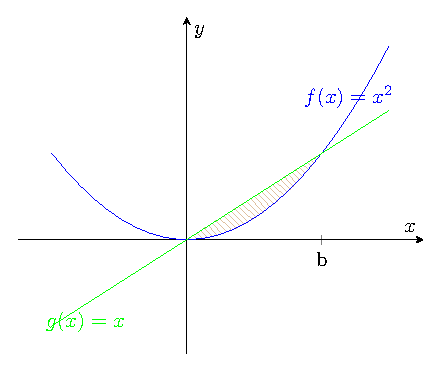
\includegraphics[width=0.5\textwidth]{areax2x.pdf}
    \end{center}

Es tallen en els punts $(0,0)$ i $(1,1)$, ja que
\[
  x^2=x \Rightarrow x^2-x=0 \Rightarrow x(x-1)=0
\]

La integració haurà de tenir en compte que la variable $x$ depèn de la $y$ i viceversa, per trobar el volum de l'objecte de la figura:

\begin{center}
  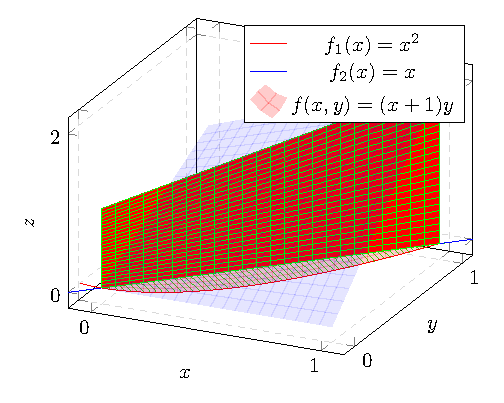
\includegraphics[width=0.5\textwidth]{volum3Dxx2xmes1y.pdf}
\end{center}

Per tant, una manera de solucionar el problema és:
\begin{eqnarray*}
V=\int \int_S (x+1)y dx dy &=& \int_{x=0}^{x=1} \left[ \int_{y=x^2}^{y=x} (x+1)y dy \right]dx \\
&=& \int_{x=0}^{x=1} \left[ \frac{(x+1)y^2}{2} \right]_{x^2}^{x} dx \\
&=& \frac{1}{2}\int_{x=0}^{x=1} \left[ (x+1)x^2 - (x+1)x^4 \right] dx\\
&=& \frac{1}{2}\int_{x=0}^{x=1} \left[ -x^5-x^4+x^3+x^2  \right] dx\\
&=& \frac{1}{2} \left[ -\frac{x^6}{6}-\frac{x^5}{5}+\frac{x^4}{4}+\frac{x^3}{3}\right]_{x=0}^{x=1}\\
&=& \frac{1}{2}\left[ \left(-\frac{1}{6}-\frac{1}{5}+\frac{1}{4}+\frac{1}{3}\right)-\left(0\right)\right]=\frac{13}{120}
\end{eqnarray*}


%\end{Answer}

\Exercise[title={Integral delimitada entre funcions}]

%\begin{Exercise}[label=Ex7]

Sigui $R$ la regió delimitada  per les corbes $f(x)=x^2+2x-3$, $g(x)=3x+3$. 
\begin{itemize}
  
  \item Representeu gràficament la regió $R$.
  \item Determineu l'àrea $A(R)$ de la regió $R$.
  \item Calculeu $\int \int_R x dxdy$ .
\end{itemize}


%\end{Exercise}

\Answer

%  \begin{Answer}[ref=Ex7]
\begin{itemize}
  \item 
Comencem per dibuixar les dues funcions.

    \begin{center}
      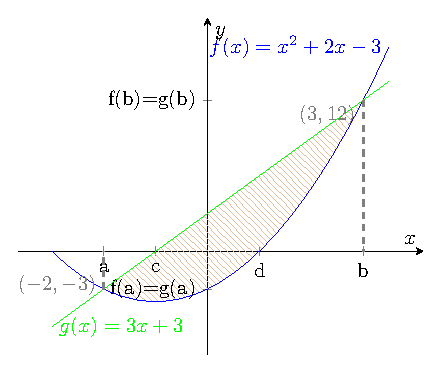
\includegraphics[width=0.5\textwidth]{areax2plus2xminus33xplus3.pdf}
    \end{center}

A partir de solucionar 
\[
  x^2+2x-3=3x+3
\]
trobem que es tallen en els punts $(-2,-3)$ i $(3,12)$.

\item Per trobar l'àrea podem pensar en dividir el càlcul en tres parts, 
si ens fan dubtar els signes de les funcions:

\[
  A(R)=\int_a^c [f(x)-g(x)] dx +  \int_c^d [g(x)+f(x)] dx + \int_d^b [g(x)-f(x)] dx
\]

o bé, més pràctic, podem sumar un valor superior a 4 a les dues funcions per tal que ens quedin les dues damunt de l'eix de les abscisses.\footnote{Només cal trobar el mínim de la funció parabòlica que es dona quan $f'(x)=2x+2=0$, que passa a $x=-1$, on $f(x)=-4$.}
Per tant, l'àrea serà igual a
\[
  A(R) = \int_a^b [(g(x)+4)-(f(x)+4)] dx = \int_a^b [g(x)-f(x)] dx 
  \] 
  \[
    A(R) = \int_{-2}^{3} [(3x+3)-(x^2+2x-3)] dx =  \int_{-2}^{3} [-x^2+x+6] dx = \left[-\frac{x^3}{3}+\frac{x^2}{2}+6x\right]_{-2}^3= \frac{125}{6}
    \] 
  
\item Com que ens donen dues funcions de la variable $x$, el més pràctic és integrar primer respecte $y$ i despreś respecte $x$:

\begin{eqnarray*}
V=\int \int_R x dx dy &=& \int \int_R x dy dx\\
&=& \int_{x=-2}^{x=3} \left[ \int_{x^2+2x-3}^{3x+3} x dy \right]dx  \\
&=& \int_{x=-2}^{x=3} x [(3x+3)-(x^2+2x-3)] dx \\
&=& \left[-\frac{x^4}{4}+\frac{x^3}{3}+3x^2\right]_{-2}^3\\
&=& \left(-\frac{3^4}{4}+\frac{3^3}{3}+3^3\right)-\left(-\frac{(-2)^4}{4}+\frac{(-2)^3}{3}+3 (-2)^2\right)
=\frac{125}{12}
\end{eqnarray*}
\end{itemize}


%\end{Answer}


\subsection{Integració de moltes variables}

\Exercise[title={Volum esfera}]
%\begin{Exercise}[label=Ex7]

  Calcula el volum d'una esfera de radi $a$ usant una integral triple.

%\end{Exercise}

\Answer

El volum de l'esfera ve donat per l'expressió:

\[
  V=\int\int\int_{\Omega} dV 
\]



Si explorem el problema usant coordenades cartesianes, l'element de volum és $\dif V= \dif x \dif y \dif z$ i els límits d'integració quedarien com:

\[
  V=\int_{-a}^a  \int_{-\sqrt{a^2-x^2}}^{\sqrt{a^2-x^2}} \int_{-\sqrt{a^2-x^2-y^2}}^{\sqrt{a^2-x^2-y^2}} \dif z \dif y \dif x 
\]

Alternativament, podem observar que la simetria de l'objecte ens permet usar coordenades esfèriques:

\begin{center}
  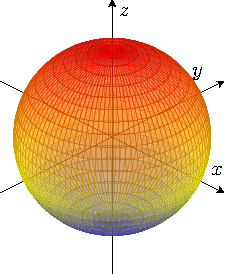
\includegraphics[width=0.3\linewidth]{sphere.pdf}
  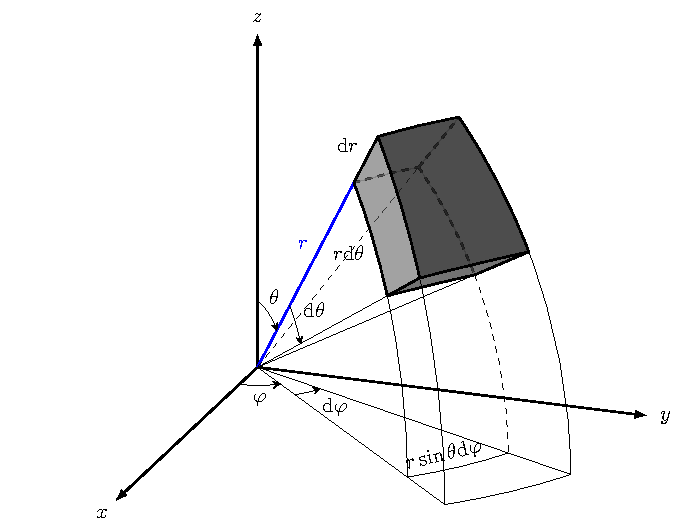
\includegraphics[width=0.6\linewidth]{CoordinatesSpherical.pdf}
\end{center}

Ara l'element de volum vindrà donat per $\dif V = r^2 \sin{\theta} \dif r \dif \theta \dif \varphi$ i els límits d'integració canviaran de forma molt favorable, ja que:

\[
\begin{cases}
  -a \leq x \leq a\\
  -\sqrt{a^2-x^2} \leq y \leq \sqrt{a^2-x^2} \\
  0 \leq z \leq a^2-x^2 - y^2\\
\end{cases}  
\Rightarrow
\begin{cases}
  0 \leq \theta \leq \pi\\
  0 \leq r \leq a \\
  0 \leq \varphi \leq 2\pi\\
\end{cases}  
\]

Així:

\begin{eqnarray*}
  V&=&\int_{0}^{2\pi}  \int_{0}^{\pi} \int_0^{a} r^2 \sin{\theta} \dif r \dif \theta \dif \varphi = \int_{0}^{2\pi} \dif \varphi  \int_{0}^{\pi} \sin{\theta} \dif \theta \int_0^{a} r^2  \dif r   \\
  &=& [\varphi]_0^{2\pi} \left[-\cos{\theta}\right]_0^{\pi} \left[\frac{r^3}{3}\right]_0^a =\boxed{\frac{4}{3}\pi a^3}
\end{eqnarray*}

%\end{Answer}

\Exercise[title={Volum paraboloide}]
%\begin{Exercise}[label=Ex7]

  Calcula el volum delimitat pel paraboloide $z=x^2+y^2$. i el pla $z=1$.

%\end{Exercise}

\Answer

Dibuixem primer el gràfic:

\begin{center}
  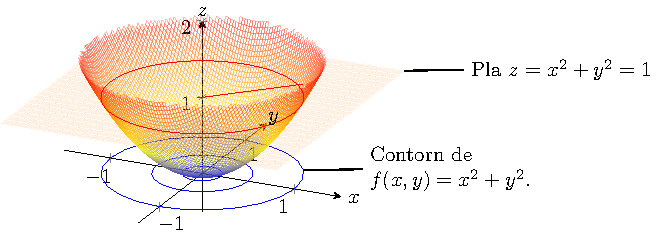
\includegraphics[width=0.9\linewidth]{paraboloid.pdf}
\end{center}

El volum del paraboloide vindria donat per l'expressió:

\[
  V=\int\int\int_{\Omega} dV 
\]

Si explorem el problema usant coordenades cartesianes, l'element de volum és $\dif V= \dif x \dif y \dif z$ i els límits d'integració quedarien com:

\[
  V=\int_{-1}^1  \int_{-\sqrt{1-x^2}}^{\sqrt{1-x^2}} \int_0^{x^2+y^2} \dif z \dif y \dif x 
\]

Podem intentar fer aquesta integral, però clarament el fet que apareguin arrels en els límits d'integració no facilita gens la feina (tot i que la integral no és pas molt complicada). Pots solucionar-la amb \texttt{Matlab} usant aquest breu codi:
\begin{lstlisting}[language=Matlab]
 syms x y z
 intZ = int(1,z,0,x^2+y^2)
 intY = int(intZ,y,-sqrt(1-x^2),sqrt(1-x^2))
 intX=int(intY)
 volum = int(intY,x,-1,1)
\end{lstlisting}

Alternativament, podem observar que la simetria de l'objecte ens permet usar coordenades cilíndriques, molt més pràctiques:

\begin{center}
  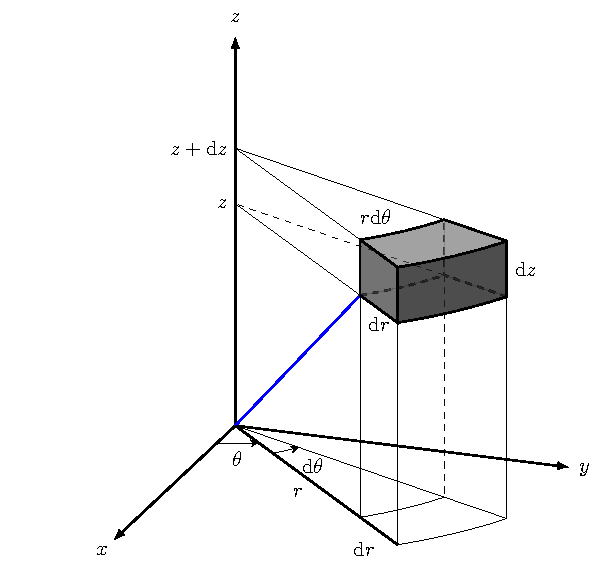
\includegraphics[width=0.5\linewidth]{CoordinatesCylindrical.pdf}
\end{center}

Ara l'element de volum vindrà donat per $\dif V = r \dif z \dif r \dif \theta$ i els límits d'integració canviaran de forma molt favorable, ja que:

\[
\begin{cases}
  -1 \leq x \leq 1\\
  -\sqrt{1-x^2} \leq y \leq \sqrt{1-x^2} \\
  0 \leq z \leq x^2 + y^2\\
\end{cases}  
\Rightarrow
\begin{cases}
  0 \leq \theta \leq 2 \pi\\
  0 \leq r \leq 1 \\
  0 \leq z \leq x^2 + y^2 = r^2\\
\end{cases}  
\]

Així:

\begin{eqnarray*}
  V&=&\int_{0}^{2\pi}  \int_{0}^{1} \int_0^{r^2} r \dif z \dif r \dif \theta = \int_{0}^{2\pi} \dif \theta  \int_{0}^{1} r \left[\int_0^{r^2} \dif z\right] \dif r \\
  &=& \theta]_{0}^{2\pi} \int_{0}^{1} r z]_0^{r^2} \dif r = 2\pi \left[\frac{r^4}{4}\right]_0^1=\boxed{\frac{\pi}{2}}
\end{eqnarray*}

%\end{Answer}


\end{ExerciseList}

\end{document}
